\documentclass[arhiv]{izpit}
\usepackage{fouriernc}
\usepackage{tikz}

\begin{document}

\izpit{Programiranje I: 2.\ izpit}{17.\ februar 2012}{
  Čas reševanja je 120 minut.
  Doseženih 100 točk šteje za maksimalno oceno.
  Veliko uspeha!
}

%%%%%%%%%%%%%%%%%%%%%%%%%%%%%%%%%%%%%%%%%%%%%%%%%%%%%%%%%%%%%%%%%%%%%%
\naloga[25 + 10 točk]

Za dano zaporedje števil $a_0, \ldots, a_{n-1}$ in naravno število $k$ je zaporedje
\emph{tekočih povprečij širine $k$} novo zaporedje $b_0, \ldots, b_{n-k}$, kjer je $b_i$
povprečje elementov $a_i, \ldots, a_{i+k-1}$.

\podnaloga[25 točk] Sestavite funkcijo
\texttt{naloga1a(a, k)}, ki sprejme tabelo števil \texttt{a} in število \texttt{k}
ter vrne tabelo tekočih povprečij širine \texttt{k} za tabelo \texttt{a}. Na primer:
%
\begin{verbatim}
>>> naloga1a([1, 2, 3, 4, 5, 6], 2)
[1.5, 2.5, 3.5, 4.5, 5.5]
>>> naloga1a([1, 2, 3, 4, 5, 6], 1)
[1.0, 2.0, 3.0, 4.0, 5.0, 6.0]
>>> naloga1a([1, 2, 3, 4, 5, 6], 6)
[3.5]
\end{verbatim}

\podnaloga[10 točk]
Sestavite funkcijo \texttt{naloga1b(a, b)}, ki sprejme tabelo \texttt{a} dolžine $k-1$ in
tabelo \texttt{b}. Znano je, da je \texttt{b} tabela tekočih povprečij širine $k$ za
tabelo, ki se začne z elementi iz tabele \texttt{a}. Funkcija naj vrne tabelo, iz katere
smo izračunali \texttt{b}. Primer:
%
\begin{verbatim}
>>> naloga1b([1.0], [1.5, 2.5, 3.5, 4.5, 5.5])
[1.0, 2.0, 3.0, 4.0, 5.0, 6.0]
>>> naloga1b([1.0, 2.0, 3.0, 4.0, 5.0], [3.5])
[1.0, 2.0, 3.0, 4.0, 5.0, 6.0]
\end{verbatim}

% def naloga1a(a,k):
%     return [sum(a[i:i+k])/k for i in range(0, len(a)-k+1)]

% def naloga1b(sez, povprecja):
%     k = len(sez) + 1
%     skoraj_povprecje = sum(sez)
%     for i, povprecje in enumerate(povprecja):
%         naslednji = k * povprecje - skoraj_povprecje
%         skoraj_povprecje += naslednji - sez[i]
%         sez.append(naslednji)
%     return sez

%%%%%%%%%%%%%%%%%%%%%%%%%%%%%%%%%%%%%%%%%%%%%%%%%%%%%%%%%%%%%%%%%%%%%%
\naloga[20 + 20 točk]

Podatkovna struktura \emph{cikel} je usmerjen krožni seznam elementov, v katerem ima vsak element vrednost in naslednika:
%
\[
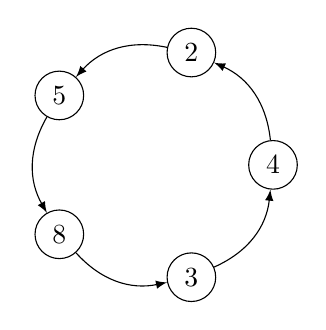
\begin{tikzpicture}
    \node (a) [circle, draw, minimum size=0.5cm] at (0 : 1.5) {4};
    \node (b) [circle, draw, minimum size=0.5cm] at (72 : 1.5) {2};
    \node (c) [circle, draw, minimum size=0.5cm] at (144 : 1.5) {5};
    \node (d) [circle, draw, minimum size=0.5cm] at (216 : 1.5) {8};
    \node (e) [circle, draw, minimum size=0.5cm] at (288 : 1.5) {3};
    \draw[bend right, >=latex, ->] (a) to (b);
    \draw[bend right, >=latex, ->] (b) to (c);
    \draw[bend right, >=latex, ->] (c) to (d);
    \draw[bend right, >=latex, ->] (d) to (e);
    \draw[bend right, >=latex, ->] (e) to (a);
\end{tikzpicture}
\]
%
Cikel predstavimo z razredom \texttt{Cikel}, ki je zapisan v datoteki na Tomotu.
%
% class Cikel:
%     def __init__(self, sez=[]):
%         self.prazen = True
%         for x in sez:
%             self.dodaj(x)
%             self = self.naslednji
%    
%     def __repr__(self):
%         if self.prazen:
%             return "()"
%         else:
%             x = self
%             vrednosti = [str(self.vrednost)]
%         while x.naslednji != self:
%             x = x.naslednji
%             vrednosti.append(str(x.vrednost))
%         return "({0})".format(", ".join(vrednosti))
%  
%     def dodaj(self, x):
%         if self.prazen:
%             self.prazen = False
%             self.vrednost = x
%             self.naslednji = self
%         else:
%             naslednji = Cikel([x])
%             self.naslednji, naslednji.naslednji = naslednji, self.naslednji
%
Cikel na zgornji sliki predstavimo takole:
%
\begin{verbatim}
>>> Cikel([4, 2, 5, 8, 3])
(4, 2, 5, 8, 3)
\end{verbatim}

\podnaloga[20 točk]
Razredu \texttt{Cikel} dodajte metodo \texttt{naloga2a(self)}, ki vrne dolžino cikla.

\podnaloga[20 točk]
Razredu \texttt{Cikel} dodajte metodo \texttt{naloga2b(self)}, ki obrne smer cikla in ne vrne
ničesar. Metoda naj ne spreminja vrednosti temveč le naslednike.

% def naloga2a(self):
%     if self.prazen:
%         return 0
%     else:
%         dolzina = 1
%         x = self
%         while x.naslednji != self:
%             x = x.naslednji
%             dolzina += 1
%         return dolzina

% def naloga2b(self):
% if self.prazen:
%     pass
% else:
%     x = self
%     y = self.naslednji
%     while y != self:
%         z = y.naslednji
%         y.naslednji = x
%         x = y
%         y = z
%     self.naslednji = x

%%%%%%%%%%%%%%%%%%%%%%%%%%%%%%%%%%%%%%%%%%%%%%%%%%%%%%%%%%%%%%%%%%%%%%
\naloga[30 točk]

V \emph{Mathematici} sestavite funkcijo \texttt{naloga3[n\_]}, ki nariše sliko, kot je prikazana na spodnjih slikah:

\begin{center}
\begin{tabular}{c@{\hspace{1.5cm}}c@{\hspace{1.5cm}}c}
  
\includegraphics[width=4cm]{kaca2.pdf}&
  
\includegraphics[width=4cm]{kaca5.pdf}&
  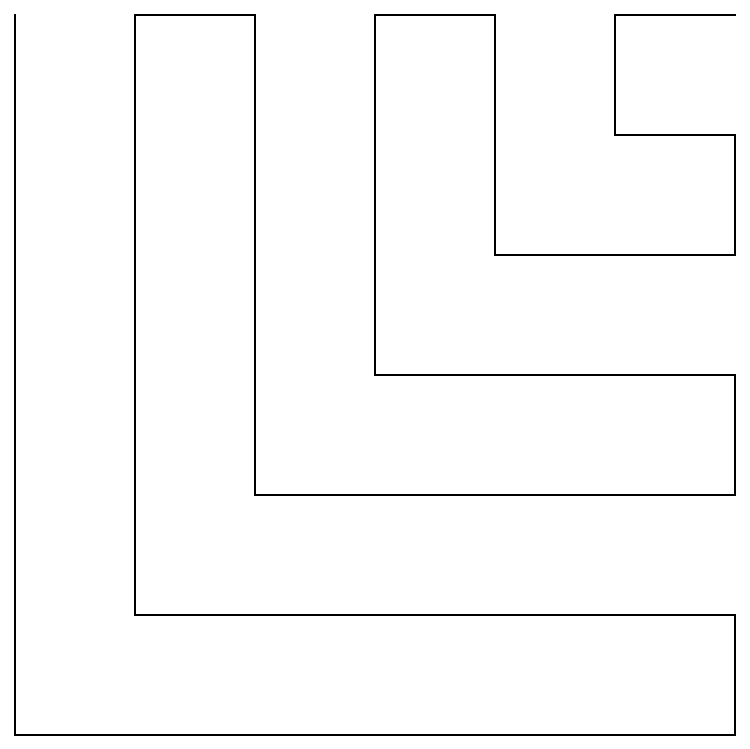
\includegraphics[width=4cm]{kaca6.pdf}\\
  \texttt{naloga3[2]} &
  \texttt{naloga3[5]} &
  \texttt{naloga3[6]}
\end{tabular}
\end{center}

% naloga3[n_] := Graphics[{
%    Table[Line[{{-k, 0}, {-k + 1, 0}}], {k, 1, n, 2}],
%    Table[Line[{{0, -k}, {0, -k + 1}}], {k, 2, n, 2}],
%    Table[Line[{{-k, 0}, {-k, -k}, {0, -k}}], {k, 1, n}]}]

\end{document}

